\section{Empirical Results}\label{results}

In this section, we proceed to present our findings. We have adopted a data window spanning 122 days to estimate Value-at-Risks (VaRs). Subsequently, we compare these estimations with the realized returns to assess the effectiveness of our methodology. To evaluate our approach, we have formulated a random portfolio comprising 100 call options and employed a buy-and-hold strategy until the options reach maturity. While alternative strategies are available, we have opted for this one due to its simplicity. The data on the options covers the period from January 3rd to June 27th of 2013. However, it is essential to note that other time frames can also be considered. Our portfolio has been meticulously designed to account for various moneyness shifts across different maturity dates. 

In Figure \ref{fig:Portfolio_PnL_Total}, the top bar plot illustrates the portfolio's return over the studied period, while its distribution of returns is depicted to the right. It is worth noting that the returns distribution is right-skewed, as the downside is limited to -100\%. At the bottom of the figure, the 90\% and 95\% VaR are outlined using the PSP method. It is important to note that a 99\% confidence level is not included in our analysis due to insufficient data. Figure \ref{fig:Portfolio_PnL_day4} illustrates a sample of the generated distribution of PnL for a randomly selected date employing the PSP method\footnote{The code was executed on an Apple M1 processor, requiring approximately 12,500 seconds for completion.}. 
\begin{figure*}
    \centerline{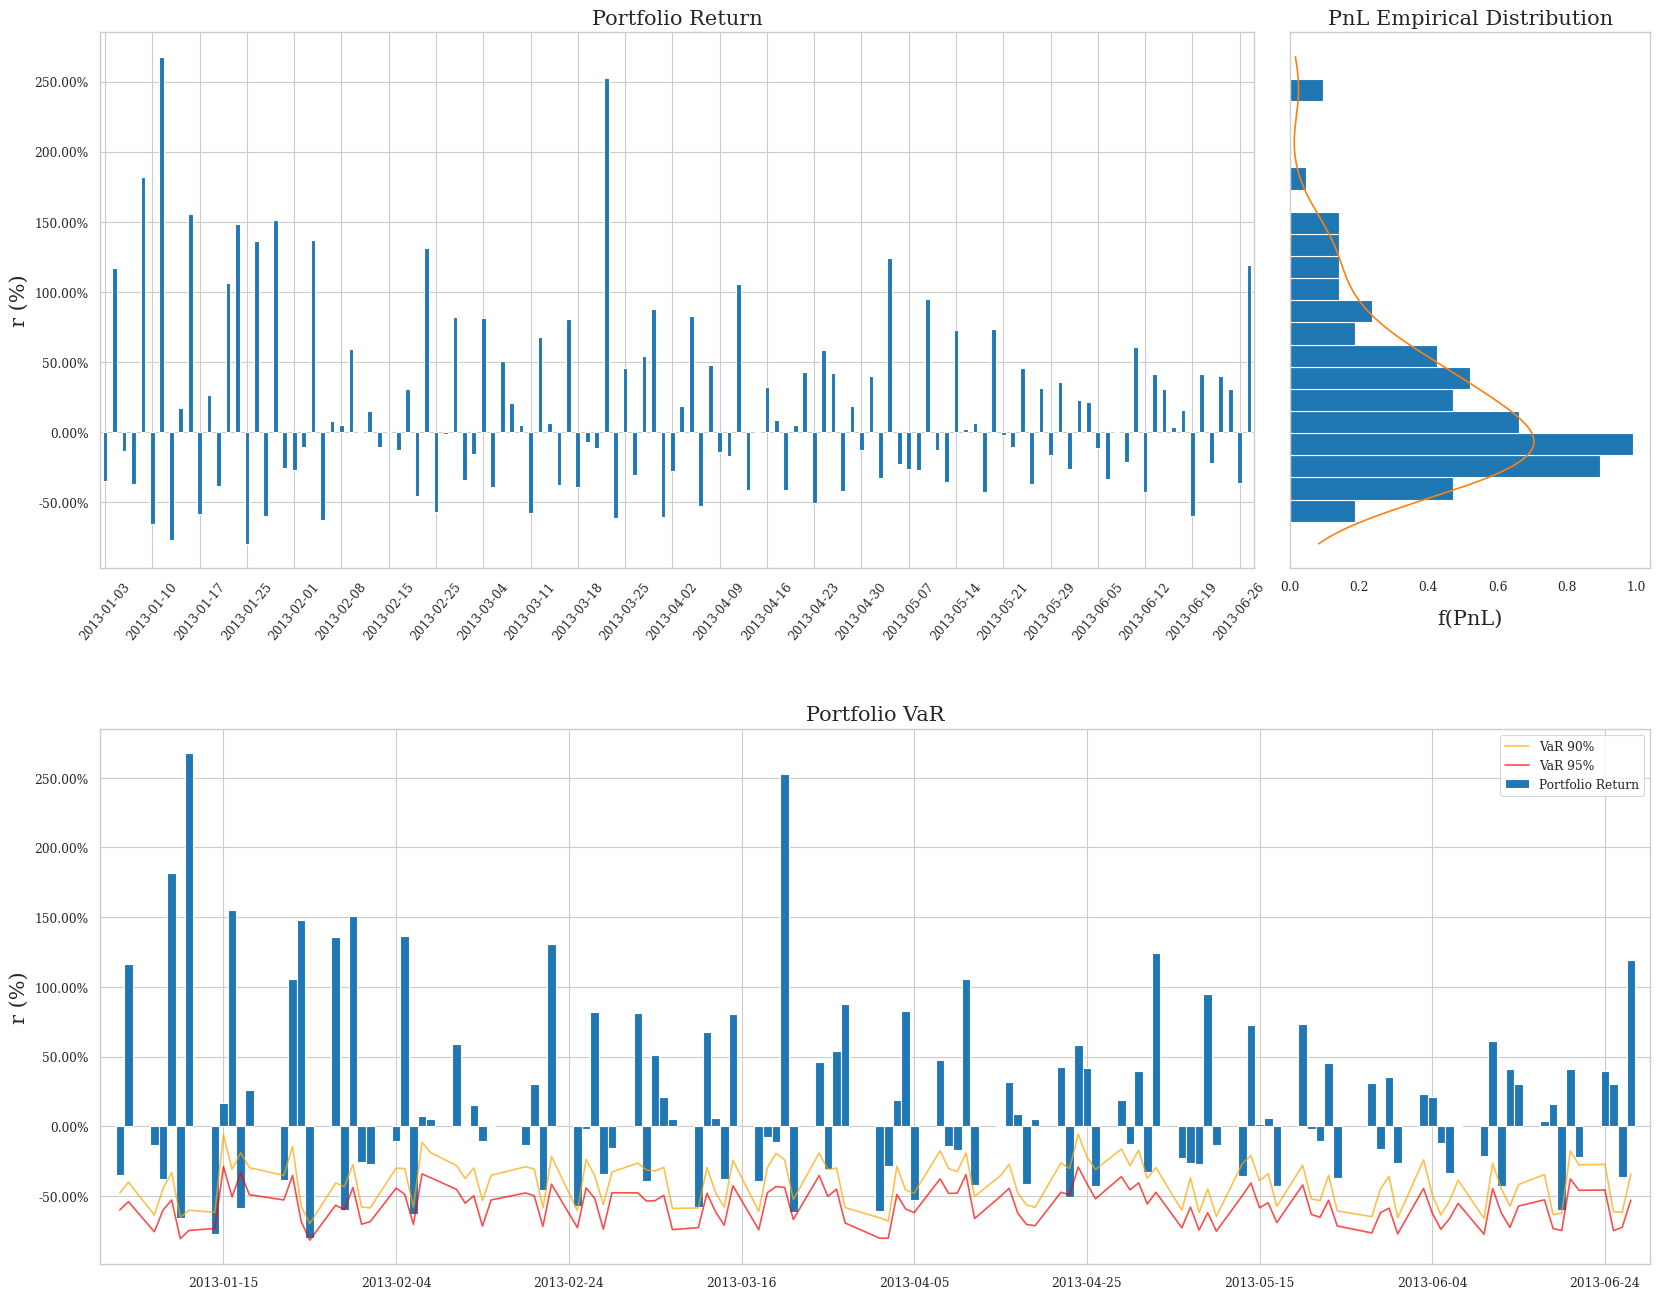
\includegraphics[width=\linewidth]{figs/PortfolioPnLTotalnew.png}}
    \caption{This figure illustrates the proposed hierarchy of VaR calculation methods within option portfolios, as introduced in the introduction. It is important to note that the hierarchy does not imply any temporal precedence of one method over another. Instead, it visually represents how our suggested model relates to other methods in this context.}
    \label{fig:Portfolio_PnL_Total}
\end{figure*}
\begin{figure}[pos=ht!]
    \centerline{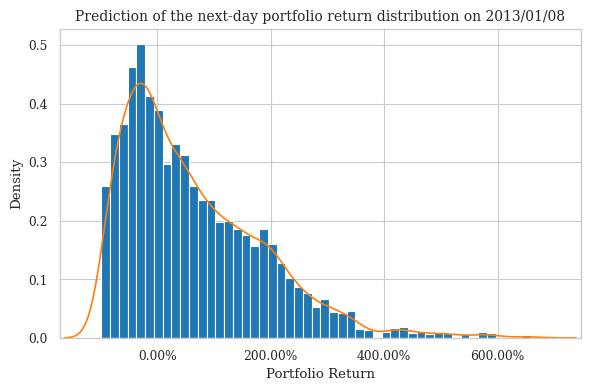
\includegraphics[width=\linewidth]{figs/PortfolioPnLdist_singledaynew.png}}
    \caption{This figure illustrates a sample of the generated distribution of Profit and Loss (PnL) for a randomly selected date using the PSP method.}
    \label{fig:Portfolio_PnL_day4}
\end{figure}

\subsection{Statistical tests to evaluate Value-at-Risk (VaR) Models}\label{sec:VaR-backtesting}

The first test is the unconditional coverage test, which evaluates the efficacy of a Value-at-Risk (VaR) calculation technique by examining the frequency of its breaches concerning the specified VaR confidence level. The second test, the independence test (\cite{roccioletti2015backtesting}), assesses whether the VaR violations demonstrate independent clustering or dispersion patterns across time. Finally, the conditional coverage test integrates components from the preceding two tests. These tests independently evaluate the dependability of each method and do not entail direct comparisons among them. Acknowledging that rejecting the null hypothesis in these tests indicates the insufficiency of a particular approach is crucial.

\begin{figure*}
    \centerline{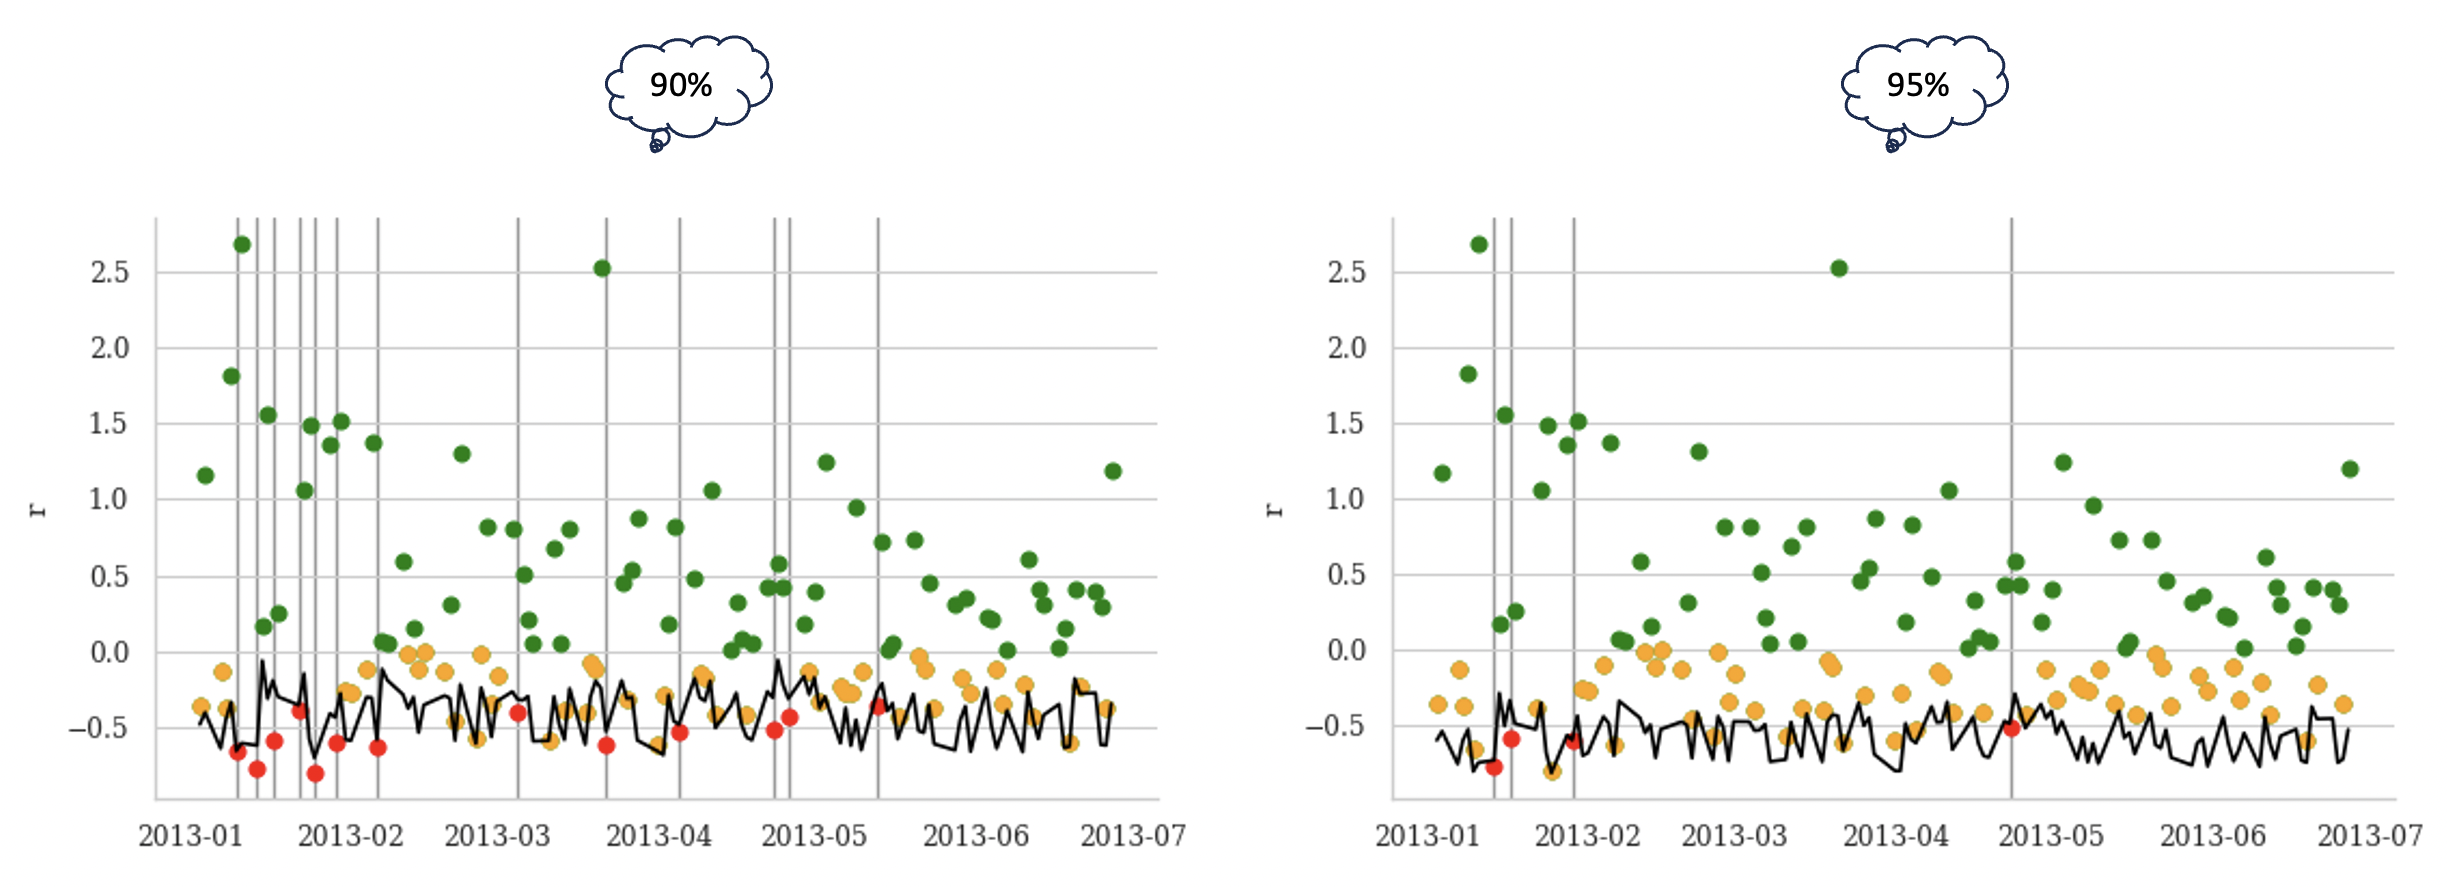
\includegraphics[width=\linewidth]{figs/PSPR1.png}}
    \caption{This figure illustrates various confidence levels associated with VaR calculated using the PSP method. The dots represent portfolio returns for each day, with green indicating positive returns, yellow for negative returns, and red for returns exceeding VaR levels.}
    \label{fig:PSP_R1}
\end{figure*}
\begin{table*}
\begin{center}
\begin{tabular}{*9c}
\hline 
\hline
\toprule
Confidence & Method & \multicolumn{2}{p{2cm}}{\centering Conditional Coverage \\ Test} & \multicolumn{2}{p{2cm}}{\centering Independence \\ Test} & \multicolumn{2}{p{2cm}}{\centering Unconditional Coverage \\ Test} & \multicolumn{1}{p{1.2cm}}{\centering Violation \\ Rate} \\
\cline{3-8}
           &        & Stat.        & P-Value & Stat.& P-Value & Stat. & P-Value &   \\
\hline
90\%    & PSP    & 3.21    & 0.2009 & 3.14  & 0.0765 & 0.07  & 0.7873 & 0.1066    \\
    & Const. Vol & 2.87    & 0.2386 & 1.13  & 0.2870 & 1.73  & 0.1881 & 0.0656    \\
    & VIX        & 3.63    & 0.1626 & 0.86  & 0.3537 & 2.77  & 0.0959 & 0.0574    \\
\hline
95\%    & PSP    & 1.10    & 0.5770 & 0.27  & 0.6010 & 0.83  & 0.3634 & 0.0328    \\
    & Const. Vol & 6.74    & 0.0344 & 0.02  & 0.8973 & 6.72  & 0.0096 & 0.0082    \\
    & VIX        & 6.74    & 0.0344 & 0.02  & 0.8973 & 6.72  & 0.0096 & 0.0082    \\
\bottomrule
\hline
\hline
\end{tabular}
\caption{The performance of the PSP, Const. Vol and VIX methods in estimating VaR with 90\% and 95\% confidence levels are assessed through conditional coverage, unconditional coverage, and independence tests.}
\label{tab:results_tests}
\end{center}
\end{table*}
Additionally, we employed the Diebold and Mariano (DM) test (\cite{epftoolbox}) to conduct pairwise comparisons of the accuracy between different time series models. This test calculates the difference between the forecasted and actual values for each time series, utilizing a loss function. In our case, the Mean Squared Error was employed as the chosen loss function. Subsequently, a statistical test is applied to determine whether the performance of one model significantly outperforms the other.

Before delving into tables and statistical analysis, we examine the VaR calculations of different methods, illustrated in Figures\footnote{These figures are generated utilizing the GitHub repository available at the following link: \url{https://github.com/BayerSe/VaR-Backtesting}} \ref{fig:PSP_R1}, \ref{fig:Const_Vol_R1}, and \ref{fig:VIX_R1}. Each figure portrays two plots for each confidence interval. Colored dots represent realized portfolio returns: green for positive returns, yellow for negative, and red when the return surpasses the VaR calculated in black. 

These figures reaffirm the superiority of the PSP method. At the same time, violations are infrequently observed in the Const. Vol and VIX models, the PSP method exhibits a notable number of violations, enhancing the reliability of our predictions. Predictions generated by the Const Vol and VIX models tend to be more conservative than those produced by the PSP method. Consequently, these models might suit regulators, emphasizing prudent capital allocation. However, the PSP method stands out for firms seeking optimal capital utilization. The ranking model will enable a comprehensive assessment, considering both regulatory and firm-oriented objectives, for evaluating the accuracies of different models.

Table \ref{tab:results_tests} presents the outcomes of unconditional coverage, independence, and conditional coverage tests for the PSP, Const. Vol, and VIX methods. Analyzing the statistics and violation rates reveals comparable performance among all methods in a 90\% confidence interval, with the PSP method demonstrating a slightly superior violation rate. However, the PSP method outshines the other two at a higher confidence level of 95\%, highlighting its effectiveness. 
\begin{figure*}
    \centerline{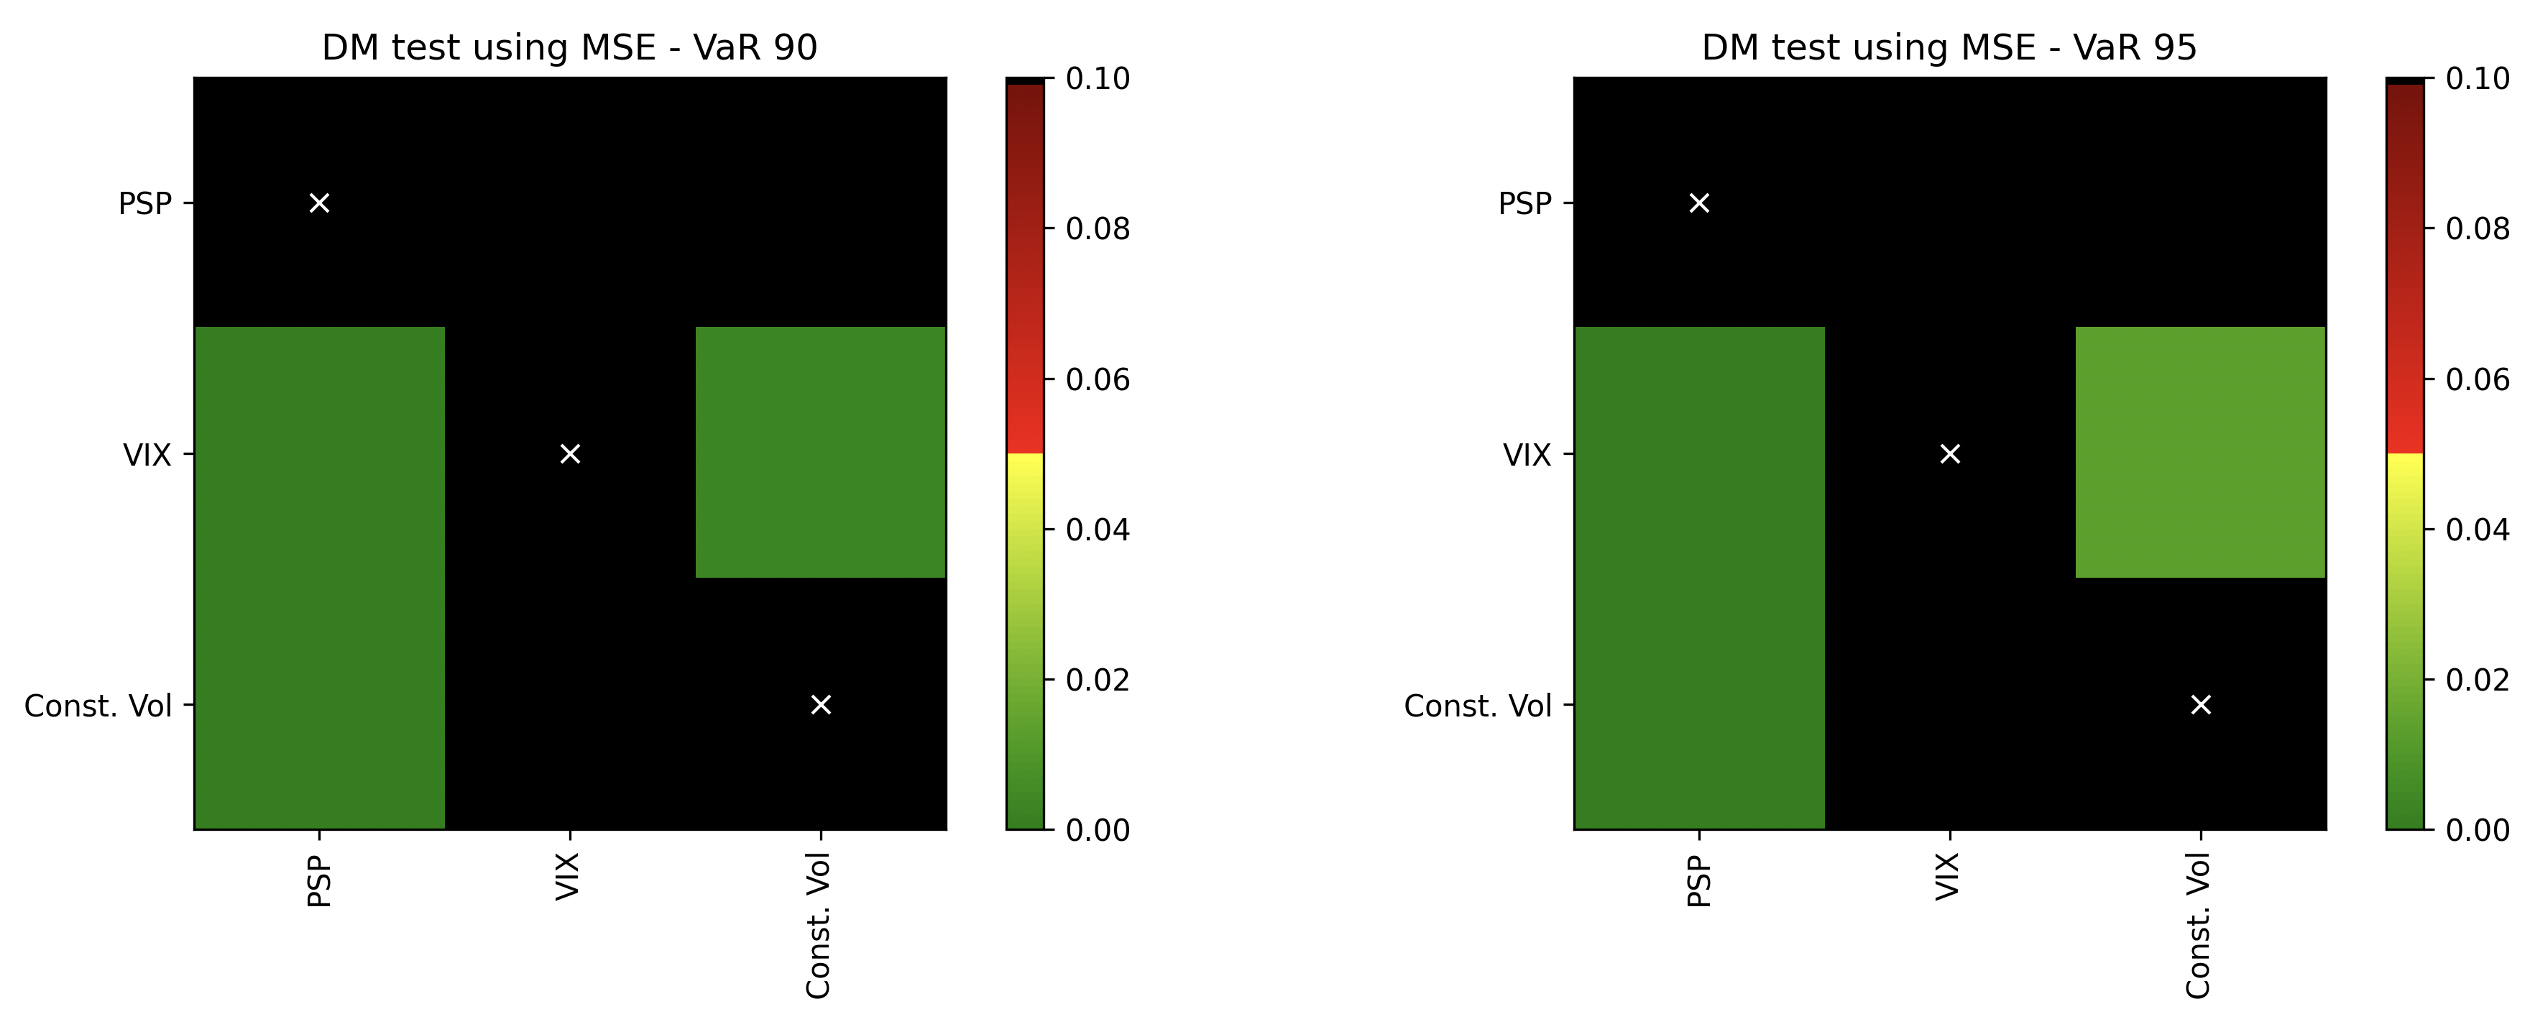
\includegraphics[width=\linewidth]{figs/DM_Test.png}}
    \caption{This figure showcases a chessboard-shaped heat map, presenting the outcomes of the Diebold and Mariano (DM) test for comparing forecasts from various models. The map reveals the p-values associated with the null hypothesis that the forecast on the y-axis is significantly more accurate than the forecast on the x-axis. Essentially, lower p-values, approaching 0, indicate instances where the forecast on the x-axis outperforms the forecast on the y-axis by a significant margin.}
    \label{fig:DM_Test}
\end{figure*}

Figure \ref{fig:DM_Test} stands out as a pivotal discovery in this study. As illustrated, the PSP method surpasses all other methods in performance. Applying the Diebold and Mariano (DM) test, employing the Mean Squared Error (MSE) as the loss function, affirms the superior accuracy of the PSP method in predictions compared to the other two methods, aligning with our expectations. Incorporating local volatilities instead of a single reference volatility proves to be a value-addition. Furthermore, the utilization of volatility, whether reference or local, demonstrates better results than not incorporating volatility at all, as seen in the Constant Volatility model. All drawn inferences hold significance, underscoring the validity of our findings.
\begin{figure*}
    \centerline{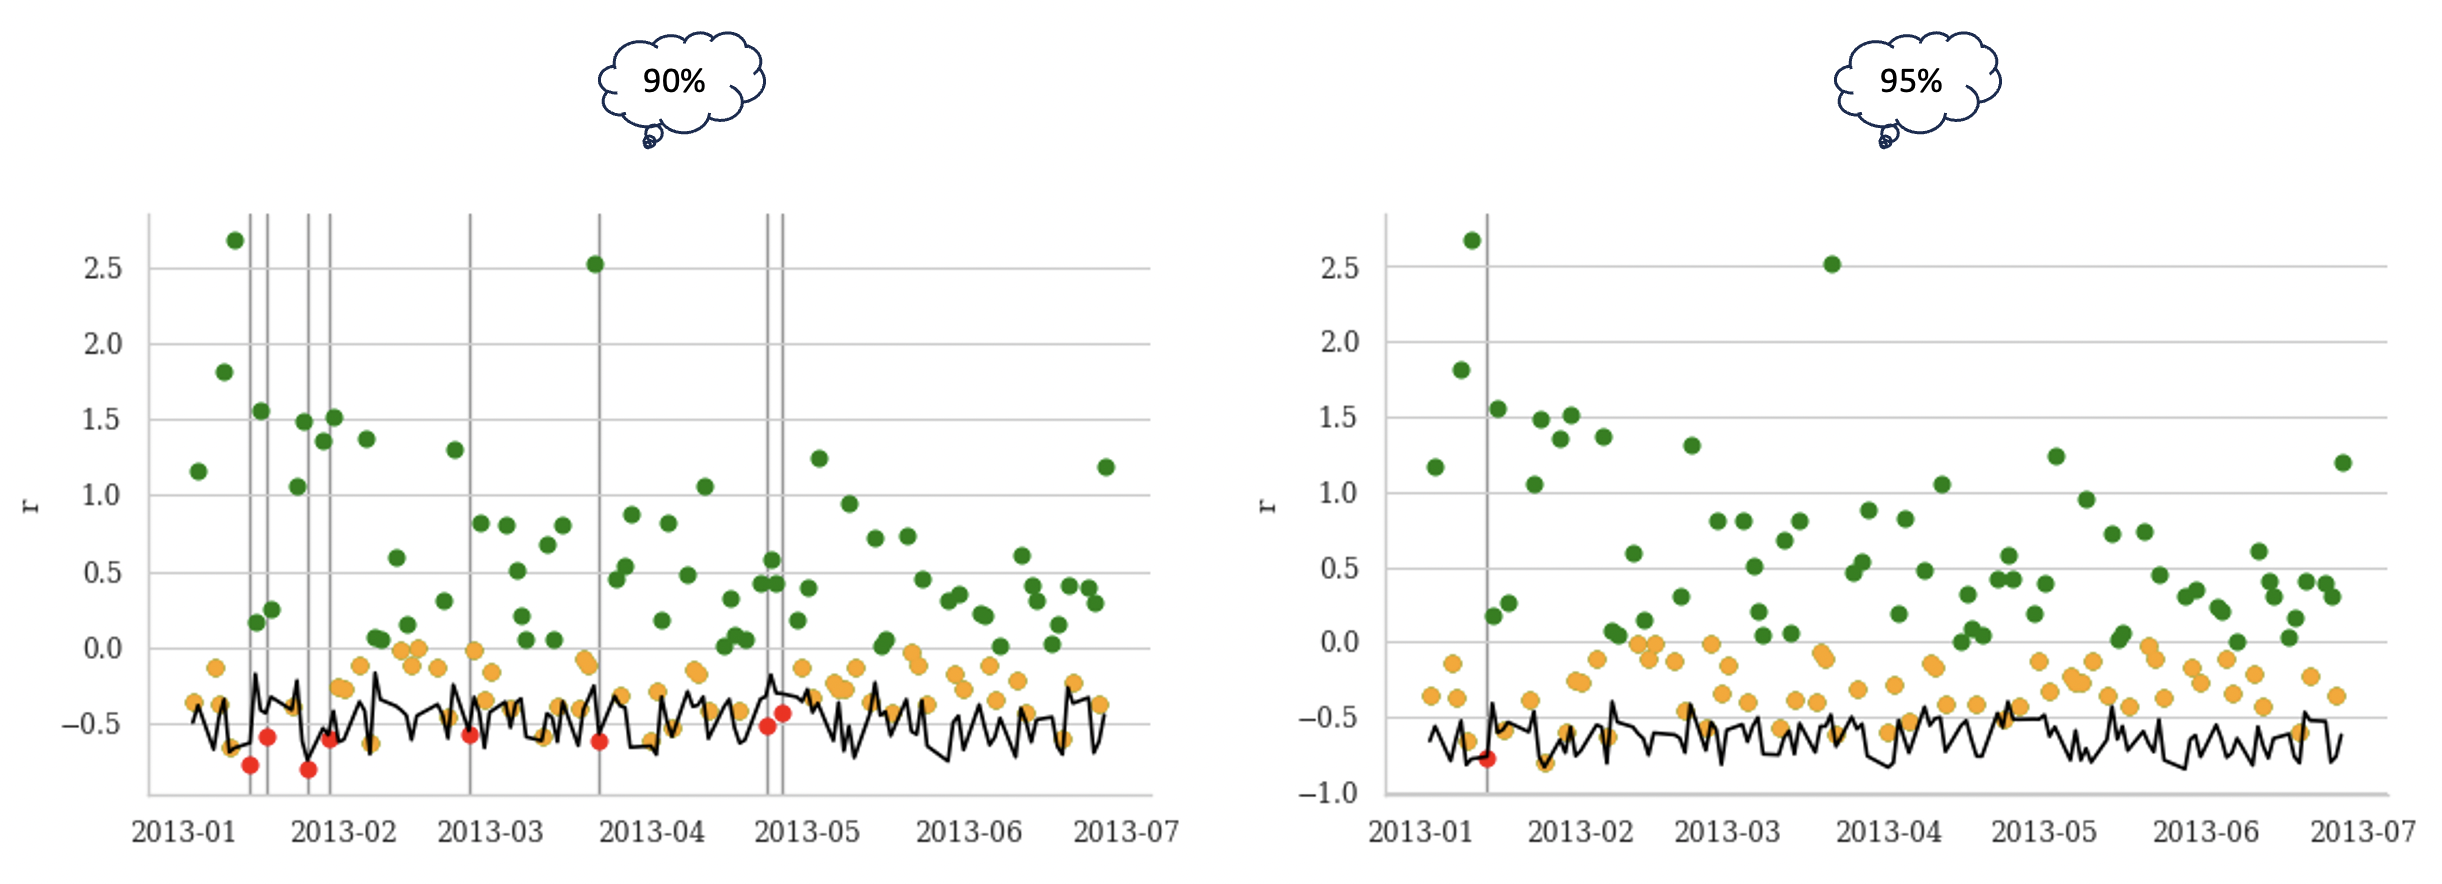
\includegraphics[width=\linewidth]{figs/ConstVolR1.png}}
    \caption{This figure illustrates various confidence levels associated with VaR calculated using the Const. Vol method. The dots represent portfolio returns for each day, with green indicating positive returns, yellow for negative returns, and red for returns exceeding VaR levels.}
    \label{fig:Const_Vol_R1}
\end{figure*}
\begin{figure*}
    \centerline{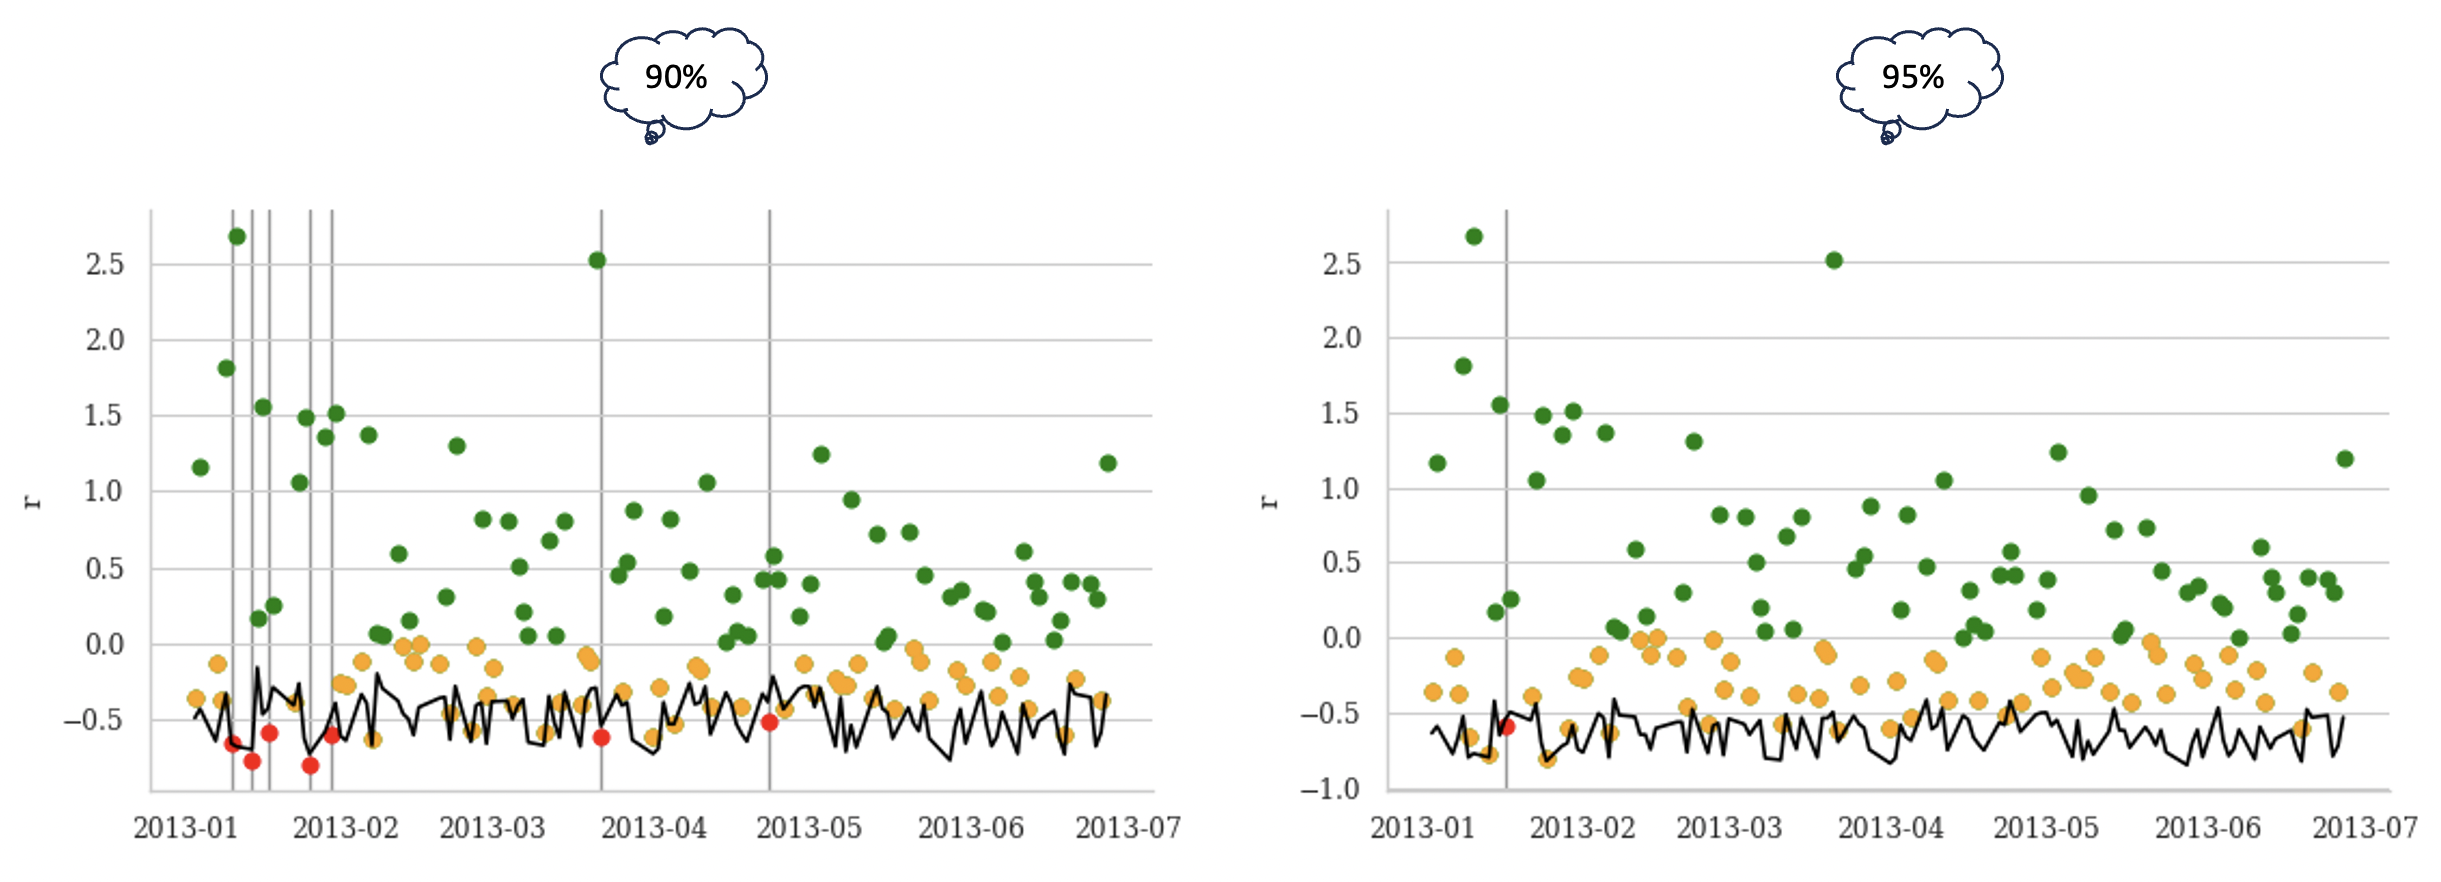
\includegraphics[width=\linewidth]{figs/VIXR1.png}}
    \caption{This figure illustrates various confidence levels associated with VaR calculated using the VIX method. The dots represent portfolio returns for each day, with green indicating positive returns, yellow for negative returns, and red for returns exceeding VaR levels.}
    \label{fig:VIX_R1}
\end{figure*}

\subsection{Performance-based Evaluation}\label{sec:Performance_based}

The Ranking Model proposed by \cite{csener2012ranking}, chosen for evaluating VaR calculation methods, introduces a penalty mechanism for each day where the forecasted VaR deviates from the realized return. The cumulative penalty across the entire period becomes instrumental in identifying the superior method. Notably, this model stands out for its unique approach—it eschews statistical tests and opts for scoring each VaR calculation method based on its performance. This characteristic allows the Ranking Model to concurrently compare several methods, setting it apart from previous models. Given our dataset's limitations for conducting robust statistical tests, the model's capacity to assess multiple methods simultaneously proves crucial for our analysis. 

Table \ref{tab:results_ranks} presents the results derived from the ranking model. Notably, the PSP method exhibits a relatively weaker performance for lower confidence intervals. This is primarily attributed to the method's higher frequency of violations. As previously discussed, the increased number of violations results in diminished accuracy from a regulatory standpoint but enhanced accuracy from a firm's perspective. In this scenario, the quantity and severity of violations lead to a lower rank for the PSP method. Conversely, the PSP method excels for higher confidence intervals, securing the top position. The fewer violations observed in the Const Vol and VIX models contribute to higher penalties, particularly from a firm's viewpoint. An intriguing observation is the relative stability of the Const Vol model, which consistently holds the second position across all confidence intervals.

\begin{table}
\begin{center}
\begin{tabular}{*5c}
\hline 
\hline
\toprule
Confidence&   Method   & Penalty & Percentage & Rank \\
\hline
90\%      & PSP        & $3.93 \times 10^{-2}$      &   38.53  & 3    \\
          & Const. Vol & $3.40 \times 10^{-2}$      &   33.33  & 2    \\
          & VIX        & $2.87 \times 10^{-2}$      &   28.14  & 1    \\
\hline
95\%      & PSP        & $1.46 \times 10^{-2}$      &   31.33  & 1    \\
          & Const. Vol & $1.54 \times 10^{-2}$      &   33.05  & 2    \\
          & VIX        & $1.66 \times 10^{-2}$      &   35.62  & 3    \\
\bottomrule
\hline
\hline
\end{tabular}
\caption{The performance of the PSP method in estimating VaR with 90\% and 95\% confidence levels is assessed through conditional coverage, unconditional coverage, and independence tests.}
\label{tab:results_ranks}
\end{center}
\end{table}

